\documentclass[12pt,a4paper]{jsarticle}
\usepackage[dvipdfmx]{graphicx}
\usepackage[dvipdfmx]{color}
\usepackage{listings}
% to use japanese correctly, install jlistings.
\lstset{
  basicstyle={\small\ttfamily},
  identifierstyle={\small},
  commentstyle={\small\itshape\color{red}},
  keywordstyle={\small\bfseries\color{cyan}},
  ndkeywordstyle={\small},
  stringstyle={\small\color{blue}},
  frame={tb},
  breaklines=true,
  numbers=left,
  numberstyle={\scriptsize},
  stepnumber=1,
  numbersep=1zw,
  xrightmargin=0zw,
  xleftmargin=3zw,
  lineskip=-0.5ex
}
\lstdefinestyle{customCsh}{
  language={csh},
  numbers=none,
}
\lstdefinestyle{customRuby}{
  language={ruby},
  numbers=left,
}
\lstdefinestyle{customTex}{
  language={tex},
  numbers=none,
}
\lstdefinestyle{customJava}{
  language={java},
  numbers=left,
}
\begin{document}
\title{卒業論文\\
\vspace{4cm} hikiutilsを用いた\\卒業論文作成}
\author{ 関西学院大学 理工学部 情報科学科\\\\1234 西谷滋人}
\date{\vspace{3cm} 2017年  3月\\
\vspace{3cm} 指導教員  西谷 滋人 教授}
\maketitle
\setcounter{tocdepth}{6}
\tableofcontents

\tableofcontents
近年,ナレッジマネジメントが企業経営の重要な要素と言われ,
導入する企業が増えている.
ナレッジマネジメントとは,個人の持つ知識や情報を組織全体で共有し,
有効に活用することで業績を上げようという経営手法である.
日本語では,「知識管理」などと訳され,「KM」と略されることもある.
参考文献1(\verb|http://e-words.jp/w/|ナレッジマネジメント.html 1/27アクセス)

ナレッジマネジメントでは,グループ開発において共有する知識は
暗黙知と形式知に分けられる.
暗黙知は主に口伝によって一対一でつたえられたり,あるいは体で覚えるというのが一般的である.
しかし,定着するまでの間は一般的にメモという形で個人的な知識として扱われるのが普通である.
一方で図書館やwebなどでは文書やhyper textとして誰もが読める形で保管,提供される.
これらは形式知と呼ばれる.

\begin{figure}[htbp]\begin{center}
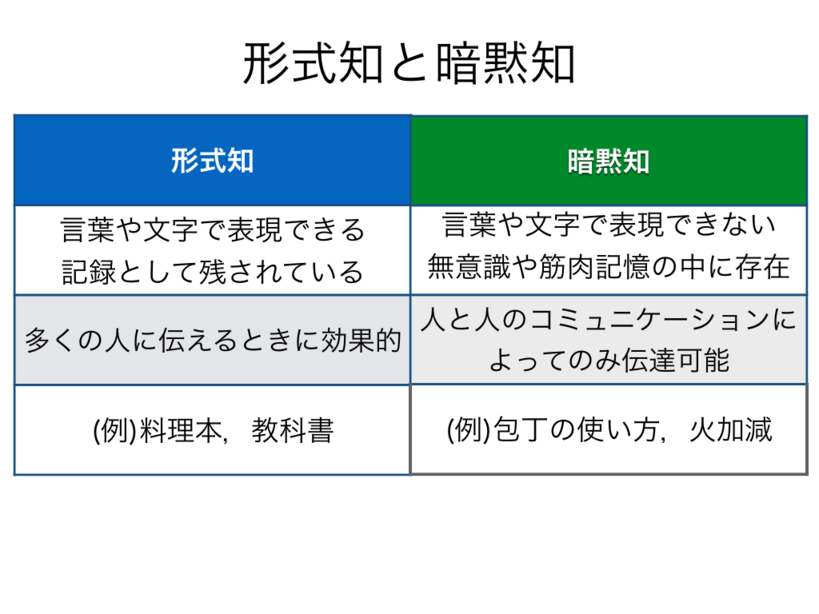
\includegraphics[width=10cm,bb= 0 0 737 453]{../figs/./my_help2hiki_saki.001.png}
\caption{暗黙知と形式知}
\label{default}\end{center}\end{figure}
参考文献2(ニック・ミルトン,「プロジェクト・ナレッジ・マネジメント」,
(生産性出版,東京都渋谷区渋谷3-1-1,2009年),p.4-5)

暗黙知の形式知化はいくつも行われている.
google検索結果でよく上位に出てくるQiita.comやcheatgraphy.comなどもそれらをまとめるサイトを提供している.
また,デザインパターンも「プログラマが持っていた暗黙知に名前をつけることで形式知化した」と
ruby開発者のまつもとゆきひろも指摘している\verb|{{fn'デザインパターン,コード解説'}}|.
ある意味,暗黙知の形式知化をいかに効率よく行うかは知識共有の最大の目的とも言える.

このような暗黙知と形式知を提供するフォーマットはそれぞれの特徴を引き出すためにそれぞれ異なった
フォーマットで記述されている.

\begin{itemize}
\item 暗黙知は主にメモとして保存しやすいように単純なテキスト形式が取られる.
\item web発信においては,複雑な構文となるhyper textではなく,手軽にwebサイトを構築するwikiに対応したmark up言語が取られる.また,
\item 書籍としては,体裁,数式の綺麗さだけでなく,目次,索引,引用文献などの自動作成の観点からlatexで書かれることが多い.
\end{itemize}
しかし,それぞれを別々に書いていては,一箇所に修正があるとすべてのフォーマットに対して行う必要が出てくる.
これはプログラマの心得の核心をなす「DRY(Don't Repeat Yourself)」原則を
破ることとなる\verb|{{fn('pragmatic programmer')}}|.
プログラマはこれらの変換を自動化するコンバータを作成して,一箇所の修正によって
他のフォーマットでの修正に反映されるように,自動的に行うシステムを構築している.

本研究においては,図2に示した通り,西谷研で活用しているメモソフト
my\_help,wiki cloneのhiki, およびlatexの間を自動変換するシステムの開発を目的としている.

\begin{figure}[htbp]\begin{center}
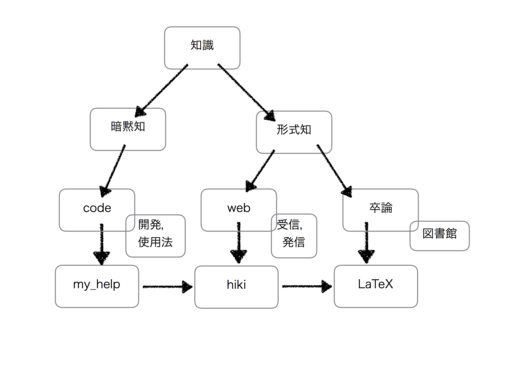
\includegraphics[width=10cm,bb= 0 0 737 453]{../figs/./knowledge_controll_cui.png}
\caption{知識の分類と,それぞれに適合したシステムおよびフォーマット.}
\label{default}\end{center}\end{figure}

\section{関連する先行研究}
\section{関連するソフトの振る舞い}
本章では,対象とするソフトはあまり一般に普及しているものではないため,
最初にソフト(my\_helpおよびhiki)の特徴と簡単な振る舞いを紹介する.

\subsection{my\_help}
my\_helpは西谷研究室で使用しているユーザ独自のメモを作成するgemである.

gemは正式名称をRubyGemsといい,
Ruby用のライブラリを使う時に必要となるソフトウェアのことである\cite{c}.
パッケージ管理ツールgemがあることで,Ruby用ライブラリの
インストール,アンインストール,バージョン管理などを簡単に
行うことができる.
プログラミング言語Rubyのファイルに付属されていて,
無料で利用することができる.

gemの利点は次の通りである。
\begin{itemize}
\item 標準化された構造があるので,初めてみた人でも分かるようになっている.
\item gemがあることで,簡単にRuby用ライブラリをインストールでき,初心者でもアプリ機能を装備できる.
\item 誰でも作成,配布が可能である.
\end{itemize}

my\_helpが提供するコマンドとその振る舞いをhelp表示から示す.
\begin{quote}\begin{verbatim}
Usage: my_help [options]
    -v, --version                    show program Version.
    -l, --list                       list specific helps
    -e, --edit NAME                  edit NAME help(eg test_help)
    -i, --init NAME                  initialize NAME help(eg test_help).
    -m, --make                       make executables for all helps.
    -c, --clean                      clean up exe dir.
        --install_local              install local after edit helps
        --delete NAME                delete NAME help
        --hiki                       my_help2hiki
\end{verbatim}\end{quote}

my\_helpではhelpの要素をこのhelp表示と同じ構造,項目と対応する記述で表示される.
それぞれの項目はまとまりをつくり,それを-lでリスト表示される.
--versionおよび--listはgem標準に準拠するために用意されている.
上記コマンドのhelp表示のNAMEには作成したhelpの名前が入る.
--edit NAMEにより,NAMEの内容を記述し更新する,--init NAMEにより,NAMEを初期化する.
exeのディレクトリを空にするには--cleanのコマンドで実行ができる.
helpを書いた後にmy\_helpによって記述や閲覧ができるようにするために,
--install\_localが用意されている.
NAMEのhelpを消したいときには,--delete NAMEによって消去ができる.
--hikiコマンドにより,my\_helpからhikiへの自動変換を行い,wikiでブラウザ表示を行う.
my\_helpを研究室内で利用する利点は次の通りである.
\begin{itemize}
\item 研究室内でのメモの書き方が統一できる.
\item どこにメモをしたか忘れることがない.
\item 普段研究の為に使うターミナルから離れること無くメモを残すことができるので,書きたいときにすぐに書くことができる.
\end{itemize}

\subsection{hiki}
hikiとは,Rubyで書かれた高機能・高速Wikiクローンである\cite{d}.
CGI(Commond Gateway Interface)を利用して,Webサーバと連動して動く\cite{e}.
西谷研究室では,hikiの形式を利用してサイトを作り,
研究室内での情報共有やgemの使い方などを掲載して閲覧できるようにしている.
また,卒業論文の作成もhikiの形式で作成している.
hikiの特徴として次のことが挙げられる.
\begin{itemize}
\item オリジナルWikiに似たシンプルな書式を持つ.
\item プラグインによる機能拡張ができる\cite{f}.
\item 携帯からアクセスが可能.
\item アクセス制限ができる.
\item 柔軟性が高く,手軽に始められて操作が簡単\cite{g}.
\item 閲覧者でも修正,ページの追加などの編集が行える.
\item 作成したページを自動で整理する\cite{h}.
\end{itemize}
これらの特徴から,複数の人が同じ情報をリアルタイムで共有し,編集しやすいという利点を持つ.
まとめサイトを作るのに適しているとして,多くのサイトに使われている.
代表的なものに百科事典であるWikipediaがある.
本研究で作成を行う西谷研究室の内部サイトも,各研究室内メンバーのメモ(暗黙知を形式知化したもの)のまとめサイトであり,
hikiを本研究に利用することは最適であるといえる.

\paragraph{hikiとは}
Rubyで書かれた高機能・高速Wikiクローン.
参考文献3(\verb|http://hikiwiki.org/ja/| 1/27)
CGI(Commond Gateway Interface)を利用して,Webサーバと連動して動く.
参考文献4(\verb|https://ja.wikipedia.org/wiki/Hiki| 1/27)
西谷研究室では,hikiの形式を利用してサイトを作り,
研究室内での情報共有やgemの使い方などを掲載して閲覧できるようにしている.
また,卒業論文の作成にもhikiの形式で作成している.


\subsubsection{TeXとは}
「テック」または「テフ」と読む,組版ソフト.
スタンフォード大学のDonald E.Knuth教授によって作られた.
他のソフトと組み合わせて,組版結果を画面や紙に出力したり,
PDF形式で出力したりする.

\subsubsection{TeXの特徴}
\begin{itemize}
\item フリーソフトなので無料で入手でき,自由に中身を調べたり改良したりできる.
\item 商品利用が自由.
\item Windows,Mac,LinuxなどのOSに関わらず同じ動作をする.
\item TeXの文書はテキストファイルなので,普通のテキストエディタで読み書きでき,再利用やデータベース化が容易.
\item 数式の組版に定評があり,数式をテキスト形式で表す標準となっている.
\end{itemize}
\subsubsection{latexとは}
「ラテック」または「ラテフ」と読む.
DEC(現在のHP)のコンピュータ科学者Leslie Lamportによって機能強化されたTeX.
もとのTeXと同様にフリーソフトとして配布されている.

参考文献5「LATEX2e 美文書作成入門」,奥村晴彦/黒木祐介著,技術評論社,2016,p.1-3


\paragraph{gem中のhikisからhikiへの自動変換}
rubyのライブラリーパッケージの標準となるgemのdirectory構造にhikisというdirectoryを作って文書作成している.hiki --initializeでこのなかのhikidocファイルをウェブ上のhikiと同期する機能を提供する.
これによって,gem/hikisで作成した文書は,githubあるいはrubygems.orgを通じて共有可能となる.
以下にこの同期をスムーズに行うための幾つかのconventionを使用法とともにまとめている.

\paragraph{使用法,コマンド}
\begin{itemize}
\item hiki --initializeで必要なファイル(Rakefile, ./.hikirc, hiki\_help.yml)がcopyされる
\item hiki\_help.ymlは適宜~/.my\_helpにcopyしてhiki\_helpとして利用\verb|my_help参照(MyHelp_install)|
\item rake syncによってhikiディレクトリーと同期が取られる
\item rake convert 20 TARGET.pngによって,figs/TAERGET.pngに20%縮小して保存される
\item hiki -u TARGETによってブラウザー表示される
\end{itemize}
\paragraph{同期に関する制約}
\begin{itemize}
\item hikiはフラットなdirectory構造を取っている
\item hikiの文書はスネーク表記(例えば,latex2hiki\_saki)で階層構造に似せている
\item hikiのurlの接頭語となる名前をbasenameのdirectory名とする.
\item directory名が'hikis'である場合はその親directory名となる.
\item ~/.hikircのtarget directoryを同期先のdirectoryとする.
\item ~/.hikircがない場合は同期先のdirectoryを聞く.
\item それらは./.hikircに保存される
\end{itemize}
\paragraph{テキスト}
\begin{itemize}
\item テキストの拡張子は'.hiki'としている
\item hikiでのurlはテキスト前とディレクトリーから自動生成される
\item 例えば,hiki2latex\_saki/introduciton.hikiとするとhiki2latex\_saki\_introducitonと変換される
\item attach\_anchorでは
\end{itemize}\begin{quote}\begin{verbatim}
'{{attach_anchor(test.png, hiki2latex_saki)}}'
\end{verbatim}\end{quote}
と,directory指定しなければならない.


\paragraph{hiki形式で書かれた文章をlatex形式に自動変換する}
\paragraph{使用法,コマンド}
\begin{itemize}
\item hiki2latex -v : hiki2latexのversion表示
\item hiki2latex -p FILE : latexの一般的なフォーマットへ変換
\item hiki2latex -b FILE :
\end{itemize}\begin{quote}\begin{verbatim}
Usage: hiki2latex [options] FILE
    -v, --version                    show program Version.
    -l, --level VALUE                set Level for output section.
    -p, --plain FILE                 make Plain document.
    -b, --bare FILE                  make Bare document.
        --head FILE                  put headers of maketitle file.
        --pre FILE                   put preamble file.
        --post FILE                  put post file.
        --listings                   use listings.sty for preformat with style.
\end{verbatim}\end{quote}
\paragraph{gem中のhikisからhikiへの自動変換}
rubyのライブラリーパッケージの標準となるgemのdirectory構造にhikisというdirectoryを作って文書作成している.hiki --initializeでこのなかのhikidocファイルをウェブ上のhikiと同期する機能を提供する.
これによって,gem/hikisで作成した文書は,githubあるいはrubygems.orgを通じて共有可能となる.
以下にこの同期をスムーズに行うための幾つかのconventionを使用法とともにまとめている.

\paragraph{使用法,コマンド}
\begin{itemize}
\item hiki --initializeで必要なファイル(Rakefile, ./.hikirc, hiki\_help.yml)がcopyされる
\item hiki\_help.ymlは適宜~/.my\_helpにcopyしてhiki\_helpとして利用\verb|my_help参照(MyHelp_install)|
\item rake syncによってhikiディレクトリーと同期が取られる
\item rake convert 20 TARGET.pngによって,figs/TAERGET.pngに20%縮小して保存される
\item hiki -u TARGETによってブラウザー表示される
\end{itemize}
\paragraph{同期に関する制約}
\begin{itemize}
\item hikiはフラットなdirectory構造を取っている
\item hikiの文書はスネーク表記(例えば,latex2hiki\_saki)で階層構造に似せている
\item hikiのurlの接頭語となる名前をbasenameのdirectory名とする.
\item directory名が'hikis'である場合はその親directory名となる.
\item ~/.hikircのtarget directoryを同期先のdirectoryとする.
\item ~/.hikircがない場合は同期先のdirectoryを聞く.
\item それらは./.hikircに保存される
\end{itemize}
\paragraph{テキスト}
\begin{itemize}
\item テキストの拡張子は'.hiki'としている
\item hikiでのurlはテキスト前とディレクトリーから自動生成される
\item 例えば,hiki2latex\_saki/introduciton.hikiとするとhiki2latex\_saki\_introducitonと変換される
\item attach\_anchorでは
\end{itemize}\begin{quote}\begin{verbatim}
'{{attach_anchor(test.png, hiki2latex_saki)}}'
\end{verbatim}\end{quote}
と,directory指定しなければならない.

my\_help2hiki\_saki\_hiki\_syncのコピー
書き換えていく


\section{my\_help,wiki,latexの自動変換システム}
\subsection{従来のmemo,latex,hiki}
\begin{figure}[htbp]\begin{center}
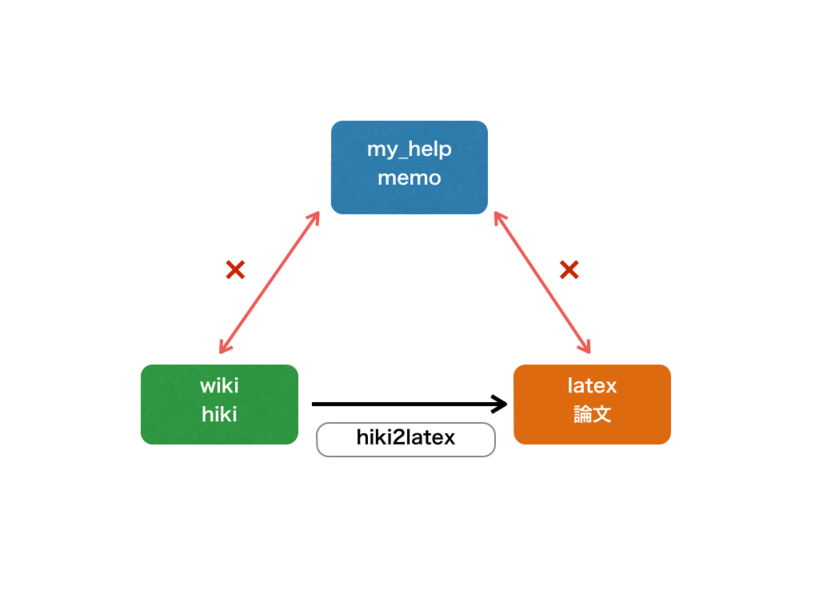
\includegraphics[width=10cm,bb= 0 0 737 453]{../figs/./my_help2hiki_saki.003.png}
\caption{ memo,latex,hikiの比較}
\label{default}\end{center}\end{figure}
\subsubsection{my\_help}
my\_helpは,メモを作るためのgem.
ユーザがターミナルを利用して作成し,閲覧する.
メモの書式はyaml形式で,拡張子は.ymlを使用している.

\subsubsection{wiki}
miというmacのテキストエディタを用いて作成する.
作成したファイルはMac OSのブラウザのsafariで開くことができる.
hiki形式で記述し,webを通して誰でも見られるようにできる.

\subsubsection{latex}
TeXの書式で,TeX編集用エディタのTeXShopによって作成する.
pdfは一般的に使われている電子ファイルで,印刷して卒業論文の
ハードコピーとしても使われる.

このようにmy\_help,wiki,latexは書式や作成,閲覧方法が全て違う.
目的も異なるので,同じ内容のファイルをそれぞれの書式で書かなければならないことがある.

\begin{figure}[htbp]\begin{center}
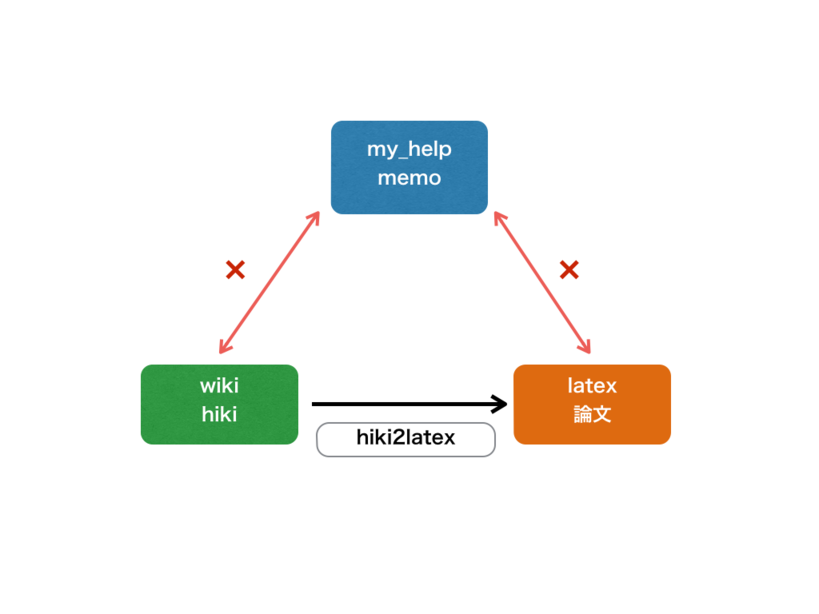
\includegraphics[width=10cm,bb= 0 0 737 453]{../figs/./my_help2hiki_saki.004.png}
\caption{ hiki2latex}
\label{default}\end{center}\end{figure}
hiki2latexの開発により上図のようにwikiとlatexの変換はできるようになったが,
my\_helpとwiki,my\_helpとlatexは関連させることができなかった.
本研究により,my\_help,wiki,latexを関連させるため,
my\_helpからwikiへ自動変換を行うシステムmy\_help2hikiの開発を目指す.

\begin{figure}[htbp]\begin{center}
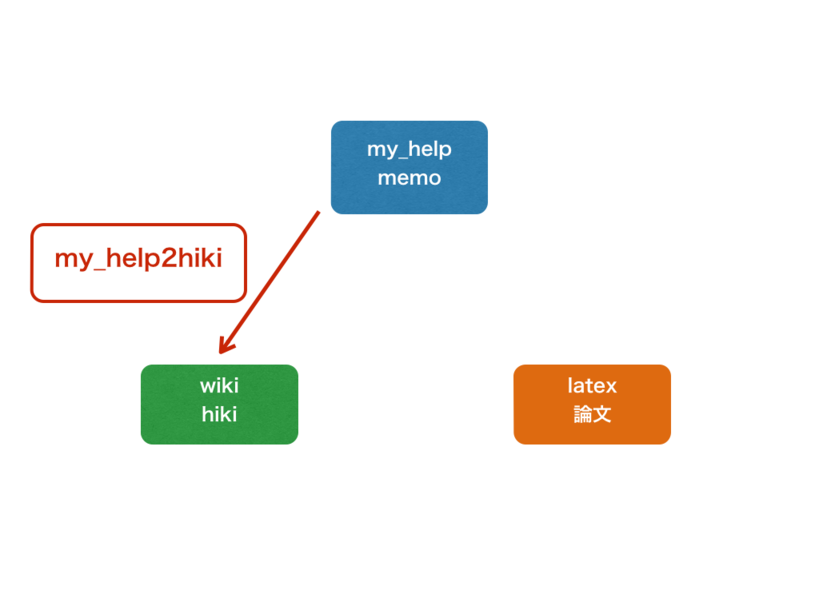
\includegraphics[width=10cm,bb= 0 0 737 453]{../figs/./my_help2hiki_saki.005.png}
\caption{my\_help2hiki}
\label{default}\end{center}\end{figure}

\include{my_help2hiki}
\section{考察}
\section{結果}
開発したmy\_helpからhikiへの自動変換を可能にするmy\_help2hiki
のコマンドと使用法,それぞれのコードについて詳述する.
また,my\_help2hikiによる利点についても記述する.

\subsection{使用法,コマンド}
my\_helpからhikiに変換するときのコマンドと使用法は以下の通りである.
\begin{itemize}
\item TARGET --push : 作成したメモ(TARGET)をサーバに送る
\end{itemize}  
\begin{itemize}
\item my\_help --hiki : 作成したメモをhiki形式に変換し,wikiで表示できるようにする.
\end{itemize}

\subsection{TARGET --push のコードの詳述}
TARGET --pushのコードについて詳述する.
振る舞いを図\ref{TARGET}に示す.
\begin{figure}[htbp]\begin{center}
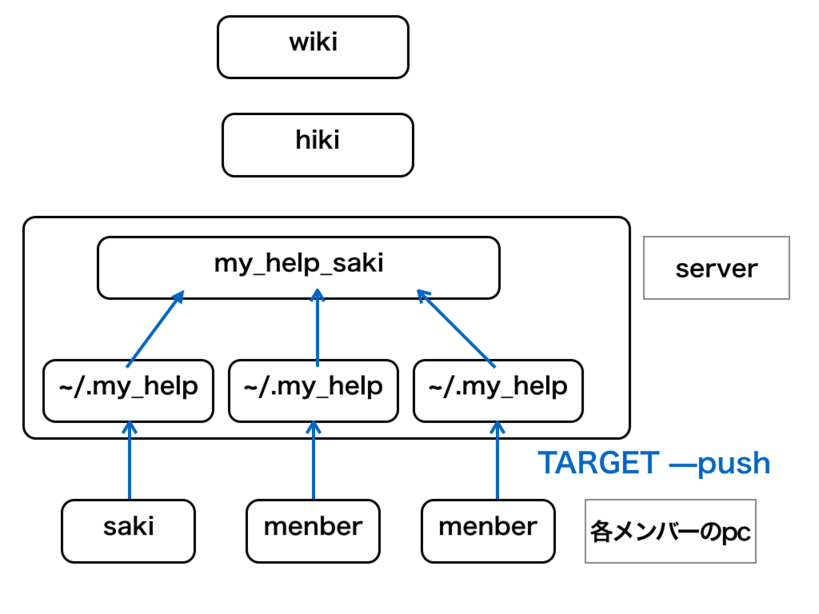
\includegraphics[width=4cm,bb=100 100 600 900]{my_help2hiki_saki.012.png}
\caption{TARGET --pushの振る舞い.}\label{TARGET}
\label{default}\end{center}\end{figure}

コードの中身は以下の通りである.
\begin{lstlisting}[style=,basicstyle={\scriptsize\ttfamily}]
    def push
      p "push my_todo"
      data_dir = File.join(ENV['HOME'],'.my_help')
      FileUtils.cd(data_dir)
      system "pwd"
      system "rm -rf ~/.my_help/*.yml~"
      system "scp -r ~/.my_help saki@nishitani0:~"
      system "ssh saki@nishitani0 ls ~/.my_help" 
    end
\end{lstlisting}
コードの詳細を記述する.

\begin{description}
\item[3,4行目]
my\_helpでは,作成したメモが.my\_helpのディレクトリに自動的に追加されるので,
ディレクトリを.my\_helpに移動する.
\end{description}

\begin{description}
\item[6行目]
.my\_helpにメモが追加されるとき,yaml形式のファイルで保存される.
メモを更新すると,一つ前に保存したファイルは*.yml~というファイル名
でバックアップとして残される.
\textbf{rm -rf}で不必要なファイルは削除し,サーバにコピーするときのデータ量を減らしている.
\end{description}

\begin{description}
\item[7行目]
\textbf{scp -r ~/[directory名] [server名]}
のコマンドによってserverにssh接続を行い,directoryをserverにコピーする.
-rはディレクトリ全体をコピーすることを示している.
西谷研究室で利用しているnishitani0というサーバにコピーしている.
\end{description}

\begin{description}
\item[8行目]
nishitani0にssh接続し.my\_helpの中身を書き出して,
コピーができているかコマンドを実行した時に確認が行えるようにしている.
\end{description}

\subsection{my\_help --hiki のコードの詳述}
my\_help --hikのコードについて詳述する.振る舞いを図\ref{--hiki}に示す.

\begin{figure}[htbp]\begin{center}
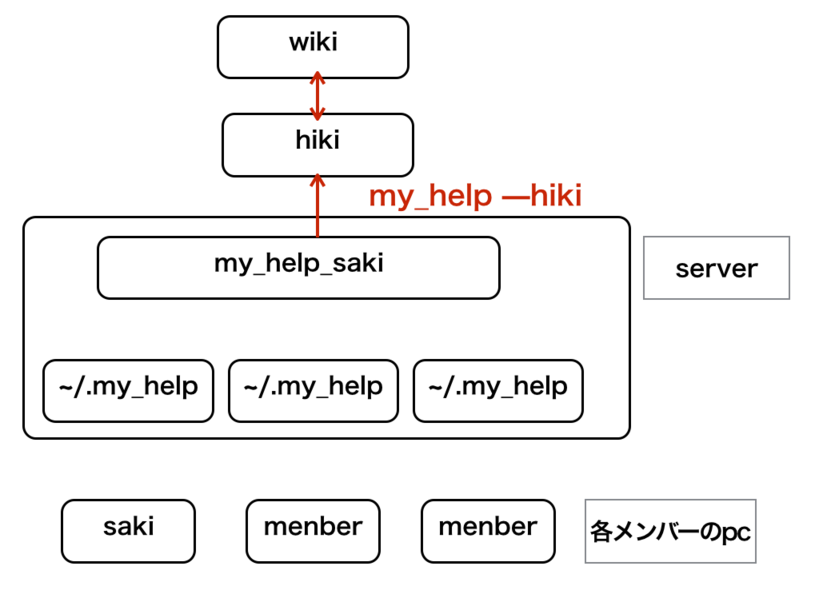
\includegraphics[width=4cm,bb=100 100 600 900]{my_help2hiki_saki.013.png}
\caption{my\_help --hikiの振る舞い.}\label{--hiki}
\label{default}\end{center}\end{figure}

コードの中身は以下の通りである.
\begin{lstlisting}[style=,basicstyle={\scriptsize\ttfamily}]
def hiki
   p 'my_help2hiki'
   system "emacs_help --to_hiki > ~/Sites/hiki-1.0/data/text/emacs_help_saki"
   system "my_todo --to_hiki > ~/Sites/hiki-1.0/data/text/my_todo_saki"
   system "ssh_help --to_hiki > ~/Sites/hiki-1.0/data/text/ssh_help_saki"
   system "open -a safari 'http://localhost/~saki/hiki-1.0/?FrontPage'"
end
\end{lstlisting}

コードの詳細について記述する.
\begin{description}
\item[3-5行目]
my\_helpには,\textbf{TARGET --to\_hiki}というコマンドがあり,これによって
yaml形式で保存されているメモをhiki形式で書き出すことができる.
この --to\_hiki のコマンドを使ってhiki形式にしたものを,wikiで表示することのできる
フォルダである\textbf{~/Sites/hiki-1.0/data/text/}に入れることで,wikiでの表示を可能にしている.
emacs\_help,my\_todo,ssh\_helpは全て私のmy\_helpに入っているメモ.
\end{description}

\begin{description}
\item[6行目]
wikiのページである,図\ref{help}に示したFrontPageを表示するコマンド.
これによりメモが更新されているのをすぐに確認することができる.
FrontPageは以下のようになっている.
\end{description}

\begin{lstlisting}[style=,basicstyle={\scriptsize\ttfamily}]
!saki's help
*[[ssh_help_saki]]
*[[my_todo_saki]]
*[[emacs_help_saki]]
\end{lstlisting}
先頭に\textbf{!}をつけることで1行目のsaki's helpを見出しにし,
2~4行目は\textbf{*}によって箇条書き,角括弧でリンクになっている.
\newpage
\begin{figure}[htbp]\begin{center}
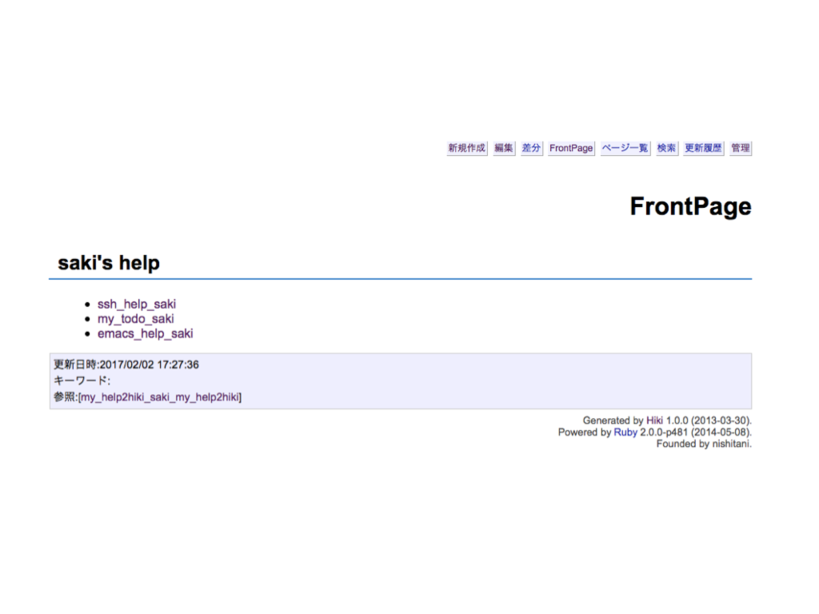
\includegraphics[clip,width=6cm,bb=100 100 600 550]{my_help2hiki_saki.002.png}
\caption{コマンドを実行したときに開くFrontPage .}\label{help}
\label{default}\end{center}\end{figure}

\subsection{my\_help2hikiによる利点}
my\_help2hikiによる利点について述べる.

\begin{lstlisting}[style=,basicstyle={\scriptsize\ttfamily}]
/Users/saki% my_help --list
Specific help file:
  emacs_help	:emacsのキーバインド
  memo_help	:ヘルプのサンプル雛形
  my_todo	:my_todo
  ssh_help	:sshのhelp
\end{lstlisting}

これは私のmy\_helpの中身を書き出している.
下がemacs\_helpの中身である.

\begin{lstlisting}[style=,basicstyle={\scriptsize\ttfamily}]
/Users/saki% emacs_help --all
emacsのキーバインド

特殊キー操作
  c-f, controlキーを押しながら    'f'
  M-f, escキーを押した後一度離して'f'
    操作の中断c-g, 操作の取り消し(Undo) c-x u
     cc by Shigeto R. Nishitani, 2016
+emacsのキーバインド:
+
特殊キー操作
+  c-f, controlキーを押しながら    'f'
+  M-f, escキーを押した後一度離して'f'
+    操作の中断c-g, 操作の取り消し(Undo) c-x u
+     cc by Shigeto R. Nishitani, 2016:
---
-カーソル移動cursor:
+c-f, move Forwrard,    前or右へ
+c-b, move Backwrard,   後or左へ
+c-a, go Ahead of line, 行頭へ
+c-e, go End of line,   行末へ
+c-n, move Next line,   次行へ
+c-p, move Previous line, 前行へ
---
---
-ページ移動page:
+c-v, move Vertical,          次のページへ
+M-v, move reversive Vertical,前のページへ
+c-l, centerise Line,       現在行を中心に
+M-<, move Top of file,    ファイルの先頭へ
+M->, move Bottom of file, ファイルの最後尾へ
---
---
-ファイル操作file:
+c-x c-f, Find file, ファイルを開く
+c-x c-s, Save file, ファイルを保存
+c-x c-w, Write file NAME, ファイルを別名で書き込む
---
---
-編集操作edit:
+c-d, Delete char, 一字削除
+c-k, Kill line,   一行抹消,カット
+c-y, Yank,        ペースト
+c-w, Kill region, 領域抹消,カット
+領域選択は,先頭or最後尾でc-spaceした後,最後尾or先頭へカーソル移動
+c-s, forward incremental Search WORD, 前へWORDを検索
+c-r, Reverse incremental search WORD, 後へWORDを検索
+M-x query-replace WORD1 <ret> WORD2:対話的置換(y or nで可否選択)
---
---
-ウィンドウ操作window:
+c-x 2, 2 windows, 二つに分割
+c-x 1, 1 windows, 一つに戻す
+c-x 3, 3rd window sep,縦線分割
+c-x o, Other windows, 次の画面へ移動
---
---
-バッファー操作buffer(すでにopenしてemacsにバッファーされたfile):
+c-x b, show Buffer,   バッファのリスト
+c-x c-b, next Buffer, 次のバッファへ移動
---
---
-終了操作quit:
+c-x c-c, Quit emacs, ファイルを保存して終了
+c-z, suspend emacs,  一時停止,fgで復活
\end{lstlisting}

このように各学生のメモを何種類も作成できるが,自分のパソコンでしか見ることができなかった.
本研究によるmy\_help2hikiを使うことで,図6のようにmy\_helpをwikiで表示可能になり,
各学生のメモを研究室内で共有することができるようになる.
今までも作成したメモをhikiに変換し,wikiで表示することは可能であったが,
メモを更新するたびにその作業をすることは手間がかかる.
本研究で開発したmy\_help2hikiを用いることで手間が省けるので,研究室内での
ナレッジマネジメントが促進されることが期待される.
\subsubsection{書き方が細かく定められている}
誤って一つでも消してしまうとエラーがでて動作しなくなってしまう.
emacs\_helpを例にする.emacs\_helpの内容は下のようになっている.
\begin{quote}\begin{verbatim}
/Users/saki/.my_help% cat emacs_help.yml
---
:head:
- "emacsのキーバインド"
- "\n特殊キー操作"
- "  c-f, controlキーを押しながら    'f'"
- "  M-f, escキーを押した後一度離して'f'"
- "    操作の中断c-g, 操作の取り消し(Undo) c-x u"
:license:
- "     cc by Shigeto R. Nishitani, 2016"
:cursor:
  :opts:
    :short: "-c"
    :long: "--cursor"
    :desc: Cursor移動
  :cont:
  - c-f, move Forwrard,    前or右へ
  - c-b, move Backwrard,   後or左へ
  - c-a, go Ahead of line, 行頭へ
  - c-e, go End of line,   行末へ
  - c-n, move Next line,   次行へ
  - c-p, move Previous line, 前行へ
:page:
  :opts:
    :short: "-p"
    :long: "--ページ"
    :desc: Page移動
  :cont:
  - c-v, move Vertical,          次のページへ
  - M-v, move reversive Vertical,前のページへ
  - c-l, centerise Line,       現在行を中心に
  - M-<, move Top of file,    ファイルの先頭へ
  - M->, move Bottom of file, ファイルの最後尾へ
  
  (以下省略)
\end{verbatim}\end{quote}
1行目の\textbf{:head:}の後ろの\textbf{:}を消してみる.
\textbf{:}を消しただけで,メモを更新しようとすると
\begin{quote}\begin{verbatim}
/Users/saki/.my_help% emacs_help --edit
/System/Library/Frameworks/Ruby.framework/Versions/2.0/usr/lib/ruby/2.0.0/psych.rb:205:in `parse': (<unknown>): mapping values are not allowed in this context at line 8 column 9 (Psych::SyntaxError)
	from /System/Library/Frameworks/Ruby.framework/Versions/2.0/usr/lib/ruby/2.0.0/psych.rb:205:in `parse_stream'
	from /System/Library/Frameworks/Ruby.framework/Versions/2.0/usr/lib/ruby/2.0.0/psych.rb:153:in `parse'
	from /System/Library/Frameworks/Ruby.framework/Versions/2.0/usr/lib/ruby/2.0.0/psych.rb:129:in `load'
	from /Library/Ruby/Gems/2.0.0/gems/my_help-0.4.3/lib/specific_help.rb:17:in `initialize'
	from /Library/Ruby/Gems/2.0.0/gems/my_help-0.4.3/lib/specific_help.rb:12:in `new'
	from /Library/Ruby/Gems/2.0.0/gems/my_help-0.4.3/lib/specific_help.rb:12:in `run'
	from /Library/Ruby/Gems/2.0.0/gems/my_help-0.4.3/exe/emacs_help:4:in `<top (required)>'
	from /usr/bin/emacs_help:23:in `load'
	from /usr/bin/emacs_help:23:in `<main>'
\end{verbatim}\end{quote}
このようになり,emacs\_helpが動かなくなってしまう.
使い慣れれば気づくことができるが,初心者ではエラーが見つけにくいと思われる.

\subsubsection{my\_helpからlatexへの変換}
\begin{figure}[htbp]\begin{center}
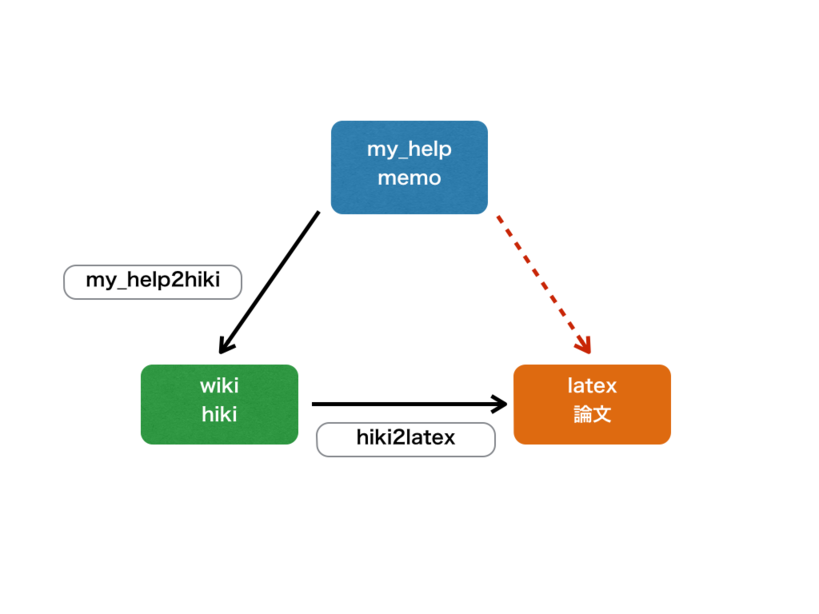
\includegraphics[width=6cm,bb=0 0 442 500]{../figs/./my_help2hiki_saki.007.png}
\caption{my\_help2hikiによるmemo,hiki,latexの関係}
\label{default}\end{center}\end{figure}
上図からも分かるように,本研究のmy\_help2hikiでも,my\_helpからlatexへ変換するには
一度hikiに変換しなければlatexへ変換することができない.

\subsubsection{コマンド}
my\_helpからhikiへの変換,hikiからlatexへの変換の操作を行うコマンドの
二つを行わなければ全てのファイルを同じ内容にすることはできない.

\subsubsection{西谷研究室の内部サイトへの表示}
西谷研究室には内部サイトがあり,研究室内で使うシステムのマニュアルなどが公開されている.
hiki形式への変換ができればwikiで表示することはできるようになるが,
my\_help2hikiのコマンドでwikiのページを作成しても,現段階では研究室内全員が見ることはできない.


先ほど記述した欠点をふまえて,
my\_help2hikiに既存システムであるhiki2latexを組み込み
\textbf{my\_help2hikiによるmemo,hiki,latexの関係}の図の破線部分にあたるシステムを作ることで,
my\_helpからlatexへとすぐに変換することのできるような,
my\_help,hiki,latexをさらに強く結びつけるシステムができるのではないかと考えている.
また,西谷研究室には内部サイトがあり,研究室内で使うシステムのマニュアルなどが公開されている.
hiki形式への変換ができればwikiで表示することはできるようになるが,
my\_helpをhikiやlatexに変換するのと同じように,その内部サイトに
各研究室生がmy\_helpによって作成したmemoを表示できるコマンドを追加すれば,
さらに便利なシステムになると考えられる.


\end{document}
